%=========== ΛΥΣΗ - 6ο ΔΙΑΓΩΝΙΣΜΑ ΠΡΟΣΟΜΟΙΩΣΗΣ ===========
\begin{thema}{Α}
\begin{erwthma}
\item Από τον ορισμό της παραγώγου έχουμε
\begin{align*}
(f+g)'(x_0)
&=\lim_{x\to x_0}\frac{(f+g)(x)-(f+g)(x_0)}{x-x_0}\\
&=\lim_{x\to x_0}\frac{f(x)+g(x)-f(x_0)-g(x_0)}{x-x_0}\\
&=\lim_{x\to x_0}\left[
\frac{f(x)-f(x_0)}{x-x_0}
+\frac{g(x)-g(x_0)}{x-x_0}
\right].
\end{align*}
Επειδή οι $f,g$ είναι παραγωγίσιμες στο $x_0$, τα δύο όρια υπάρχουν. Άρα
\[
(f+g)'(x_0)=f'(x_0)+g'(x_0).
\]
Επομένως η $f+g$ είναι παραγωγίσιμη στο $x_0$ και ισχύει
\[
{(f+g)'(x_0)=f'(x_0)+g'(x_0)}.
\]

\item Το σημείο $A(x_0,f(x_0))$ λέγεται σημείο καμπής της γραφικής παράστασης της $f$, όταν η $f$ είναι συνεχής στο $x_0$ και η γραφική της παράσταση αλλάζει κυρτότητα εκατέρωθεν του $x_0$.

\item Η ευθεία
\[
y=y_0
\]
λέγεται οριζόντια ασύμπτωτη της γραφικής παράστασης μιας συνάρτησης $f$ στο $+\infty$, όταν
\[
\lim_{x\to+\infty}f(x)=y_0.
\]

\item Οι χαρακτηρισμοί είναι:
\begin{alist}
\item \textbf{Σωστό}. Από το Θεμελιώδες Θεώρημα του Ολοκληρωτικού Λογισμού,
\[
\dint_a^\beta f'(x)\,\d x=f(\beta)-f(a).
\]
\item \textbf{Σωστό}. Κάθε γνησίως μονότονη συνάρτηση είναι $1-1$, άρα αντιστρέφεται στο σύνολο τιμών της.
\item \textbf{Λάθος}. Αν δύο συναρτήσεις έχουν ίσες παραγώγους σε διάστημα, τότε διαφέρουν κατά σταθερά, δεν είναι υποχρεωτικά ίδιες.
\item \textbf{Λάθος}. Ισχύει
\[
\dint_a^a f(x)\,\d x=0
\]
για κάθε $a$, όχι μόνο για $a=0$.
\item \textbf{Σωστό}. Αν η $f$ είναι δύο φορές παραγωγίσιμη και κοίλη σε διάστημα $\varDelta$, τότε ισχύει $f''(x)\leq0$ σε κάθε εσωτερικό σημείο του $\varDelta$.
\end{alist}
\end{erwthma}
\end{thema}

\begin{thema}{Β}
Δίνεται η συνάρτηση
\[
f(x)=(x-1)e^{-x},\quad x\in\mathbb{R}.
\]
\begin{erwthma}
\item Η $f$ είναι συνεχής στο $\mathbb{R}$, άρα δεν έχει κατακόρυφες ασύμπτωτες.

Στο $+\infty$ έχουμε
\[
\lim_{x\to+\infty}f(x)
=\lim_{x\to+\infty}\frac{x-1}{e^x}
\xlongequal[\text{\eng{DLH}}]{\frac{+\infty}{+\infty}}
\lim_{x\to+\infty}\frac{1}{e^x}=0.
\]
Άρα η ευθεία
\[
{y=0}
\]
είναι οριζόντια ασύμπτωτη της $C_f$ στο $+\infty$.

Στο $-\infty$ έχουμε
\[
\lim_{x\to-\infty}(x-1)e^{-x}=-\infty,
\]
οπότε δεν υπάρχει οριζόντια ασύμπτωτη στο $-\infty$.

\item Για κάθε $x\in\mathbb{R}$ είναι
\begin{align*}
f'(x)&=(x-1)'e^{-x}+(x-1)(e^{-x})'\\
&=e^{-x}-(x-1)e^{-x}\\
&=e^{-x}(2-x).
\end{align*}
Επειδή $e^{-x}>0$, το πρόσημο της $f'$ είναι το πρόσημο του $2-x$:
\begin{itemize}
\item $f'(x)=0\Leftrightarrow x=2$.
\item $f'(x)>0\Leftrightarrow x<2$.
\item $f'(x)<0\Leftrightarrow x>2$.
\end{itemize}
Στον παρακάτω πίνακα βλέπουμε τα πρόσημα της $f'$ και τη μονοτονία της $f$:
\begin{center}
\begin{tikzpicture}
\tkzTabInit[color,lgt=2,espcl=1.5,colorC = maincolor!50!white,colorL = maincolor!20!white,colorV = maincolor!50!white]%
{$x$ /0.8,$f'(x)$ /0.8,$f(x)$/0.8}%
{$-\infty$,$2$,$+\infty$}%
\tkzTabLine{,+,z,-,}
\tkzTabLine{,\nearrow,t,\searrow,}
\end{tikzpicture}
\end{center}
Άρα η $f$ είναι \textbf{γνησίως αύξουσα} στο $(-\infty,2]$ και \textbf{γνησίως φθίνουσα} στο $[2,+\infty)$.

Επομένως παρουσιάζει ολικό μέγιστο στο $x=2$, με τιμή
\[
f(2)=e^{-2}=\frac{1}{e^2}.
\]

\item Από το προηγούμενο ερώτημα
\[
f'(x)=e^{-x}(2-x).
\]
Άρα
\begin{align*}
f''(x)&=(e^{-x})'(2-x)+e^{-x}(2-x)'\\
&=-e^{-x}(2-x)-e^{-x}\\
&=e^{-x}(x-3).
\end{align*}
Επειδή $e^{-x}>0$, το πρόσημο της $f''$ είναι το πρόσημο του $x-3$:
\begin{itemize}
\item $f''(x)=0\Leftrightarrow x=3$.
\item $f''(x)<0\Leftrightarrow x<3$.
\item $f''(x)>0\Leftrightarrow x>3$.
\end{itemize}
Στον παρακάτω πίνακα βλέπουμε την κυρτότητα της $f$:
\begin{center}
\begin{tikzpicture}
\tkzTabInit[color,lgt=2,espcl=1.5,colorC = maincolor!50!white,colorL = maincolor!20!white,colorV = maincolor!50!white]%
{$x$ /0.8,$f''(x)$ /0.8,$f(x)$/0.8}%
{$-\infty$,$3$,$+\infty$}%
\tkzTabLine{,-,z,+,}
\tkzTabLine{,\curvearrowright,t,\rotatebox[origin= c]{180}{$\curvearrowleft$},}
\end{tikzpicture}
\end{center}
Άρα η $f$ είναι κοίλη στο $(-\infty,3]$ και κυρτή στο $[3,+\infty)$.

Η $C_f$ έχει σημείο καμπής το
\[
A(3,f(3))\equiv A\left(3,\frac{2}{e^3}\right).
\]

\item Στο διάστημα $[1,2]$ ισχύει
\[
f(x)=(x-1)e^{-x}\geq0.
\]
Άρα το ζητούμενο εμβαδόν είναι
\[
E=\dint_1^2 (x-1)e^{-x}\,\d x.
\]
Επειδή
\[
\left(-xe^{-x}\right)'=(x-1)e^{-x},
\]
έχουμε
\begin{align*}
E&=\left[-xe^{-x}\right]_1^2\\
&=-2e^{-2}+e^{-1}\\
&=\frac{1}{e}-\frac{2}{e^2}
=\frac{e-2}{e^2}.
\end{align*}
Άρα
\[
{E=\frac{e-2}{e^2}}.
\]
\end{erwthma}
\end{thema}

\begin{thema}{Γ}
Ο όγκος της κυλινδρικής κονσέρβας είναι σταθερός και ίσος με
\[
V=500\ \si{cm}^3.
\]
\begin{erwthma}
\item Για κύλινδρο ακτίνας $r$ και ύψους $h$ έχουμε
\[
V=\pi r^2h.
\]
Άρα
\[
\pi r^2h=500
\Leftrightarrow
h=\frac{500}{\pi r^2}.
\]
Το εμβαδόν των δύο βάσεων είναι
\[
2\pi r^2,
\]
οπότε το κόστος των βάσεων είναι
\[
0,02\cdot2\pi r^2=0,04\pi r^2.
\]
Το εμβαδόν της παράπλευρης επιφάνειας είναι
\[
2\pi rh=2\pi r\cdot\frac{500}{\pi r^2}=\frac{1000}{r},
\]
οπότε το κόστος της παράπλευρης επιφάνειας είναι
\[
0,01\cdot\frac{1000}{r}=\frac{10}{r}.
\]
Επομένως το συνολικό κόστος είναι
\[
{K(r)=0,04\pi r^2+\frac{10}{r}},\quad r>0.
\]

\item Για κάθε $r>0$ είναι
\[
K'(r)=0,08\pi r-\frac{10}{r^2}
=\frac{0,08\pi r^3-10}{r^2}.
\]
Επειδή $r^2>0$, το πρόσημο της $K'$ είναι το πρόσημο του
\[
0,08\pi r^3-10.
\]
Έχουμε
\[
K'(r)=0
\Leftrightarrow 0,08\pi r^3=10
\Leftrightarrow r^3=\frac{125}{\pi}
\Leftrightarrow r=\frac{5}{\sqrt[3]{\pi}}.
\]
Άρα
\[
K'(r)<0\quad\text{για }0<r<\frac{5}{\sqrt[3]{\pi}}
\]
και
\[
K'(r)>0\quad\text{για }r>\frac{5}{\sqrt[3]{\pi}}.
\]
Επομένως η $K$ είναι γνησίως φθίνουσα στο
\[
\left(0,\frac{5}{\sqrt[3]{\pi}}\right]
\]
και γνησίως αύξουσα στο
\[
\left[\frac{5}{\sqrt[3]{\pi}},+\infty\right).
\]
Άρα το συνολικό κόστος ελαχιστοποιείται μοναδικά για
\[
{r=\frac{5}{\sqrt[3]{\pi}}}.
\]

\item Θέτουμε
\[
r_0=\frac{5}{\sqrt[3]{\pi}}.
\]
Τότε
\begin{align*}
K(r_0)&=0,04\pi\cdot\frac{25}{\pi^{2/3}}+\frac{10}{5/\pi^{1/3}}\\
&=\pi^{1/3}+2\pi^{1/3}\\
&=3\sqrt[3]{\pi}.
\end{align*}
Επειδή $\pi<8$, έχουμε
\[
\sqrt[3]{\pi}<2
\]
και άρα
\[
K(r_0)=3\sqrt[3]{\pi}<6<15.
\]
Επιπλέον
\[
\lim_{r\to+\infty}K(r)=+\infty.
\]
Η $K$ είναι συνεχής στο $[r_0,+\infty)$ και γνησίως αύξουσα στο διάστημα αυτό. Επομένως, από το θεώρημα \eng{Bolzano}, υπάρχει τουλάχιστον ένα
\[
R>r_0=\frac{5}{\sqrt[3]{\pi}}
\]
τέτοιο ώστε
\[
K(R)=15.
\]

\item Από τη σχέση σταθερού όγκου
\[
\pi r^2h=500
\]
παραγωγίζουμε ως προς τον χρόνο:
\[
\pi\left(2rr'h+r^2h'\right)=0.
\]
Εναλλακτικά,
\[
h=\frac{500}{\pi r^2}.
\]
Άρα
\[
h'=-\frac{1000}{\pi r^3}r'.
\]
Τη χρονική στιγμή $t_0$ έχουμε
\[
r(t_0)=5
\quad\text{και}\quad
r'(t_0)=0,5=\frac{1}{2}.
\]
Επομένως
\[
h'(t_0)=-\frac{1000}{\pi\cdot5^3}\cdot\frac{1}{2}
=-\frac{4}{\pi}.
\]
Άρα
\[
{h'(t_0)=-\frac{4}{\pi}\ \si{cm}/\sec}.
\]
\end{erwthma}
\end{thema}

\begin{thema}{Δ}
Δίνεται παραγωγίσιμη συνάρτηση $f:\mathbb{R}\to\mathbb{R}$ με
\[
f(1)=e
\]
και
\[
f'(x)>2xf(x)
\]
για κάθε $x\in\mathbb{R}$.
\begin{erwthma}
\item Θεωρούμε τη συνάρτηση
\[
g(x)=f(x)e^{-x^2},\quad x\in\mathbb{R}.
\]
Η $g$ είναι παραγωγίσιμη και
\begin{align*}
g'(x)&=f'(x)e^{-x^2}+f(x)(e^{-x^2})'\\
&=e^{-x^2}\bigl(f'(x)-2xf(x)\bigr).
\end{align*}
Επειδή
\[
e^{-x^2}>0
\quad\text{και}\quad
f'(x)-2xf(x)>0,
\]
έχουμε
\[
g'(x)>0
\]
για κάθε $x\in\mathbb{R}$. Άρα η $g$ είναι γνησίως αύξουσα στο $\mathbb{R}$.

Για $x>1$ έχουμε
\[
g(x)>g(1)
\Leftrightarrow f(x)e^{-x^2}>f(1)e^{-1}
\Leftrightarrow f(x)e^{-x^2}>1.
\]
Άρα
\[
{f(x)>e^{x^2},\quad x>1}.
\]

\item Για κάθε $x>1$, από το προηγούμενο ερώτημα έχουμε
\[
f(x)>e^{x^2}>0.
\]
Επειδή $x>1$, ισχύει $2x>0$, άρα
\[
f'(x)>2xf(x)>0.
\]
Επομένως η $f$ είναι \textbf{γνησίως αύξουσα} στο $(1,+\infty)$.

Επιπλέον, για κάθε $x>1$,
\[
f(x)>e^{x^2}.
\]
Επειδή
\[
\lim_{x\to+\infty}e^{x^2}=+\infty,
\]
από κριτήριο σύγκρισης παίρνουμε
\[
{\lim_{x\to+\infty}f(x)=+\infty}.
\]

\item Η $f$ είναι συνεχής στο $[1,2]$ και παραγωγίσιμη στο $(1,2)$. Από το Θεώρημα Μέσης Τιμής υπάρχει $\xi\in(1,2)$ τέτοιο ώστε
\[
f'(\xi)=\frac{f(2)-f(1)}{2-1}=f(2)-f(1).
\]

Για το ίδιο $\xi$ έχουμε, από τη δοσμένη ανισότητα,
\[
f'(\xi)>2\xi f(\xi).
\]
Επειδή $\xi>1$ και από το πρώτο ερώτημα
\[
f(\xi)>e^{\xi^2}>e,
\]
παίρνουμε
\[
2\xi f(\xi)>2e.
\]
Άρα
\[
f(2)-f(1)=f'(\xi)>2e.
\]
Επομένως
\[
{f(2)-f(1)>2e}.
\]

\item Για κάθε $a>1$, από τη δοσμένη ανισότητα και το Δ1 ερώτημα έχουμε
\[
f'(a)>2af(a)>2ae^{a^2}.
\]
Άρα ο ρυθμός μεταβολής της $f$ στο σημείο με τετμημένη $a>1$ είναι αυστηρά μεγαλύτερος από
\[
{2ae^{a^2}}.
\]

Έστω, προς άτοπο, ότι υπάρχει εφαπτομένη της $C_f$ σε σημείο με τετμημένη $x_0>1$, η οποία σχηματίζει με τον άξονα $x'x$ γωνία $\omega\leq45^\circ$.

Η κλίση της εφαπτομένης είναι
\[
\lambda=f'(x_0).
\]
Από το προηγούμενο συμπέρασμα,
\[
f'(x_0)>2x_0e^{x_0^2}.
\]
Επειδή $x_0>1$, έχουμε
\[
2x_0e^{x_0^2}>2e>1.
\]
Άρα
\[
\lambda=f'(x_0)>1.
\]
Όμως, αν $\omega\leq45^\circ$, τότε
\[
\lambda=\ef\omega\leq\ef45^\circ=1,
\]
άτοπο. Επομένως δεν υπάρχει τέτοια εφαπτομένη.
\end{erwthma}
\end{thema}
%=========== ΤΕΛΟΣ ΛΥΣΗΣ - 6ο ΔΙΑΓΩΝΙΣΜΑ ΠΡΟΣΟΜΟΙΩΣΗΣ ===========
